\documentclass[preprint,12pt]{elsarticle}
\usepackage{amsmath,amssymb,amsfonts}
\usepackage{graphicx}
\usepackage{booktabs}
\usepackage{multirow}
\usepackage{xcolor}
\usepackage{hyperref}
\usepackage{algorithm}
\usepackage{algorithmic}

\journal{Expert Systems with Applications}

\begin{document}
\begin{frontmatter}

\title{TripSense-FairNet v2: Rotation-Invariant Dual-Stream Consensus, Nash Counterfactual Recourse, and Verifiably Faithful Explainable AI for Sustainable Group Travel Planning}

\author[diu]{Sabbir Hossan Sani}
\ead{sani2305101776@diu.edu.bd}
\affiliation[diu]{organization={Department of Software Engineering, Daffodil International University}, city={Dhaka}, country={Bangladesh}}

\begin{abstract}
Group travel planning presents a coupled multi-objective dilemma: maximizing collective itinerary relevance for heterogeneous companions while minimizing intra-group satisfaction inequality (Rawlsian fairness), promoting low-carbon small-and-medium enterprise (SME) destinations (provider sustainability), guaranteeing deterministic budget feasibility, and delivering auditable explanations. Existing neural group recommenders overfit to high-dimensional city-specific embedding subspaces, causing severe performance degradation under cross-city domain shift, whereas tree ensembles optimize pointwise accuracy without differentiable fairness or environmental constraints. In this work, we introduce \textbf{TripSense-FairNet v2}, a 64,286-parameter rotation-invariant dual-stream neural consensus architecture operating on mean-centered multimodal CLIP ViT-B/32 representations. Stream~1 combines rotation-invariant intra-group geometric interaction tokens with a bounded low-rank Hadamard semantic residual ($0.35\tanh(\cdot)$) and multi-head cross-attention over companions, paired with a smooth Soft-Min safety gate. Stream~2 processes a 15-dimensional city-agnostic group-relational highway without input LayerNorm distortion. We jointly optimize listwise sampled InfoNCE ($K{=}20$, $\tau{=}0.20$), a smooth pairwise Differentiable Gini regularizer augmented with Soft-Slate Rawlsian dispersion, a Least-Misery floor, and Differentiable Expected Eco-Exposure. Across a zero-leakage chronological benchmark built from \textit{Massive-STEPS-Sydney} ($29{,}900$ check-ins, $8{,}189$ venues, $1{,}200$ groups), TripSense-FairNet v2 achieves $\text{NDCG@10} = 0.5394$ ($95\%$ CI $[0.4971, 0.5810]$), $\text{Hit@10} = 0.9000$, $\text{Gini} = 0.0630$, and Top-5 Eco Coverage $= 38.67\%$, outperforming nine baselines including LightGBM ($0.4736$, Holm-Bonferroni $p = 0.00105$), GroupMLP ($0.4715$), Random Forest ($0.4520$), and AGREE ($0.4329$; Friedman $\chi^2 = 513.035$, $p = 9.291 \times 10^{-105}$). In zero-shot transfer without retraining across three unseen metropolises, FairNet v2 outperforms LightGBM in Melbourne ($0.3190$ vs.\ $0.2941$) and Tokyo ($0.3130$ vs.\ $0.2669$) and remains competitive in New-York ($0.3090$) while delivering the highest eco coverage across all external cities. Multi-paradigm XAI auditing verifies exact Integrated Gradients Completeness ($\text{MAE} = 3.0 \times 10^{-6}$), $3.43\times$ Perturbation Comprehensiveness over random masking, $0.4697$ cross-attention allocation toward lowest-budget members, and $+6.25\%$ Nash bargaining counterfactual welfare gains alongside $100.0\%$ hard budget feasibility ($0.934\text{ ms}$) across 180 \textit{TravelPlanner} tasks.
\end{abstract}

\begin{keyword}
Group Recommender Systems \sep Algorithmic Fairness \sep Explainable Artificial Intelligence \sep Zero-Shot Cross-City Transfer \sep Sustainable Tourism \sep Nash Bargaining
\end{keyword}
\end{frontmatter}

\section{Introduction}
Traveling with companions transforms individualized venue selection into a multi-party social choice problem \cite{masthoff2015group,cao2018attentive}. Members within a single travel party routinely exhibit conflicting aesthetic preferences and disparate spending capacities (e.g., Student/Budget vs.\ Mid-range vs.\ Luxury tiers). Purely utilitarian recommenders maximize mean predicted preference, systematically marginalizing budget-constrained or minority-taste companions (high satisfaction Gini inequality and low minimum member utility \cite{xiao2017fairness,kaya2020ensuring}). Conversely, rigid Least-Misery heuristics equalize dissatisfaction at the cost of sharply degraded ranking accuracy. Simultaneously, destination platforms that over-index on historical check-in popularity amplify over-tourism around congested commercial hubs while starving low-carbon community and small-and-medium enterprise (SME) providers \cite{burke2017multisided,patro2020fairrec}.

Although neural attention aggregators such as AGREE \cite{cao2018attentive} learn latent member weights, they exhibit two structural weaknesses observed in empirical cross-domain evaluation: (i) projecting high-dimensional dense embeddings ($D{=}512$) through unconstrained dense layers on modest group interaction counts causes memorization of city-specific lexical subspaces (e.g., local station names), harming zero-shot generalization when transferring from Sydney to unseen cities such as Melbourne, Tokyo, or New-York; and (ii) pointwise or pairwise BPR objectives lack explicit differentiable listwise fairness and ecological exposure gradients. Meanwhile, gradient-boosted decision trees such as LightGBM \cite{ke2017lightgbm} generalize robustly on low-dimensional relational summaries, yet remain non-differentiable with respect to companion-level attention equity and lack neural cross-attention transparency.

To bridge this gap, we propose \textbf{TripSense-FairNet v2}, embedded inside an end-to-end neuro-symbolic sustainable travel platform covering both global cross-city benchmarks and a five-city emerging-market deployment audit in Bangladesh (Dhaka, Chittagong, Sylhet, Cox's Bazar, Bandarban). Our primary contributions are:
\begin{enumerate}
    \item \textbf{Rotation-Invariant Dual-Stream Consensus Architecture:} We eliminate city-coordinate memorization via isotropic All-but-the-Top CLIP centering \cite{mu2018all} combined with rotation-invariant intra-group geometric tokens, a bounded low-rank Hadamard residual ($0.35\tanh$), and an un-squashed 15-dimensional relational highway trained under sampled InfoNCE with Differentiable Gini, Soft-Slate Rawlsian Dispersion, and Expected Eco-Exposure losses.
    \item \textbf{Multi-Paradigm Quantitative XAI Verification:} Beyond post-hoc feature weights, we verify 32-step Integrated Gradients \cite{sundararajan2017axiomatic} via Axiom~1 Completeness ($\text{MAE} = 3.0 \times 10^{-6}$), ERASER Comprehensiveness and Sufficiency \cite{deyoung2020eraser}, permutation importance, TreeSHAP cross-method concordance \cite{lundberg2017unified}, cross-attention budget equity ($0.4697$ weight allocated to lowest-budget members vs.\ $0.1728$ for highest-budget peers), and Nash Bargaining counterfactual recourse \cite{nash1950bargaining}.
    \item \textbf{Zero-Leakage Multi-City & Neuro-Symbolic Evaluation:} We demonstrate statistically significant superiority across 10 models on Sydney ($n{=}180$ test groups, 5 random seeds), zero-shot cross-city transfer across Melbourne, Tokyo, and New-York ($n{=}480$ groups total), Bangladesh 5-city equity audits, cold-start Bayesian Expected Information Gain (EIG) elicitation, and deterministic constraint verification on 180 \textit{TravelPlanner} tasks \cite{xie2024travelplanner}.
\end{enumerate}

\section{Related Work}
\textbf{Group Recommendation and Consensus Aggregation.} Early heuristic strategies aggregate individual utilities via Average, Least-Misery, or Borda Count rules \cite{masthoff2015group}. Neural models such as AGREE \cite{cao2018attentive} compute learned attention weights across member embeddings under neural collaborative filtering \cite{he2017neural}. Pareto-efficient group recommenders \cite{xiao2017fairness,kaya2020ensuring} formulate fairness via variance or rank-sensitive balancing, yet rarely couple consumer fairness with provider sustainability and cross-city domain invariance.

\textbf{Two-Sided Fairness and Sustainable Tourism.} Multi-sided fairness formalizes consumer equity alongside producer exposure \cite{burke2017multisided,patro2020fairrec}. In tourism, popularity bias concentrates visitation in saturated precincts, undermining eco-sustainability and local SME revenue dispersion \cite{chen2023bias}.

\textbf{Faithful Explainable AI and Neuro-Symbolic Planning.} Recent XAI rigor demands perturbation faithfulness checks (Comprehensiveness, Sufficiency, AOPC) alongside axiomatic attribution \cite{sundararajan2017axiomatic,deyoung2020eraser,lundberg2017unified}. Meanwhile, unconstrained language models fail severely on multi-constraint itinerary planning, achieving only $0.6\%$--$4.4\%$ final pass rates on \textit{TravelPlanner} \cite{xie2024travelplanner}, motivating deterministic constraint-satisfaction verification.

\section{Methodology}

\subsection{Zero-Leakage Chronological Formulation & Isotropic Embeddings}
Let $\mathcal{V}$ denote the venue set of a city and $\mathcal{U}$ the traveler set. Each venue $p \in \mathcal{V}$ carries a city-agnostic textual prompt $t_p = \text{``}\text{Name} \mid \text{Category}\text{''}$ encoded via frozen CLIP ViT-B/32 \cite{radford2021learning} into $\tilde{\mathbf{e}}_p \in \mathbb{R}^{512}$, followed by unsupervised All-but-the-Top centering \cite{mu2018all} $\mathbf{e}_p = (\tilde{\mathbf{e}}_p - \bar{\mathbf{e}}) / \|\tilde{\mathbf{e}}_p - \bar{\mathbf{e}}\|_2$ to eliminate narrow-cone anisotropy without touching any interaction label. Alongside semantic embeddings, each venue has an 8-dimensional city-invariant context vector $\mathbf{x}_p \in [0,1]^8$: distance centrality $d_p$, price tier $\pi_p$, log-normalized popularity $\text{pop}_p$, community rating $r_p$, indoor flag, hidden-gem indicator ($\text{pop}_p \le 0.35$), eco-sustainability score $e^{\text{eco}}_p$, and local SME share $s^{\text{sme}}_p$.

For every companion $u$ in group $G$ ($|G| \in \{2,\dots,5\}$), we partition chronological check-in trails strictly using the earliest $72\%$ as historical taste context $\mathcal{H}_u$ and strictly hold out future venues $\mathcal{Y}_G^+$ such that $\mathcal{Y}_G^+ \cap \bigcup_{u \in G} \mathcal{H}_u = \emptyset$. Companion embedding $\mathbf{e}_u$ is the $L_2$-normalized centroid of $\{\mathbf{e}_v : v \in \mathcal{H}_u\}$, paired with companion context $\mathbf{z}_u = [b_u, \text{div}_u, \text{flex}_u] \in [0,1]^3$.

\subsection{TripSense-FairNet v2 Dual-Stream Architecture}
Figure~\ref{fig:arch} illustrates the overall dual-stream architecture. Given group $G$ and candidate POI $p$, let $c_u = \langle \mathbf{e}_u, \mathbf{e}_p \rangle$ and budget hardship $\beta_u = \max(0, \pi_p - b_u)$. We construct the 15-dimensional permutation-invariant group-relational vector:
\begin{equation}
\mathbf{r}_{G,p} = \big[\bar{c}_G,\; c^{\min}_G,\; c^{\max}_G,\; \sigma(c_G),\; \bar{\beta}_G,\; \beta^{\max}_G,\; \tfrac{|G|}{5},\; \mathbf{x}_p^\top \big]^\top \in \mathbb{R}^{15}.
\end{equation}

\begin{figure}[t]
\centering
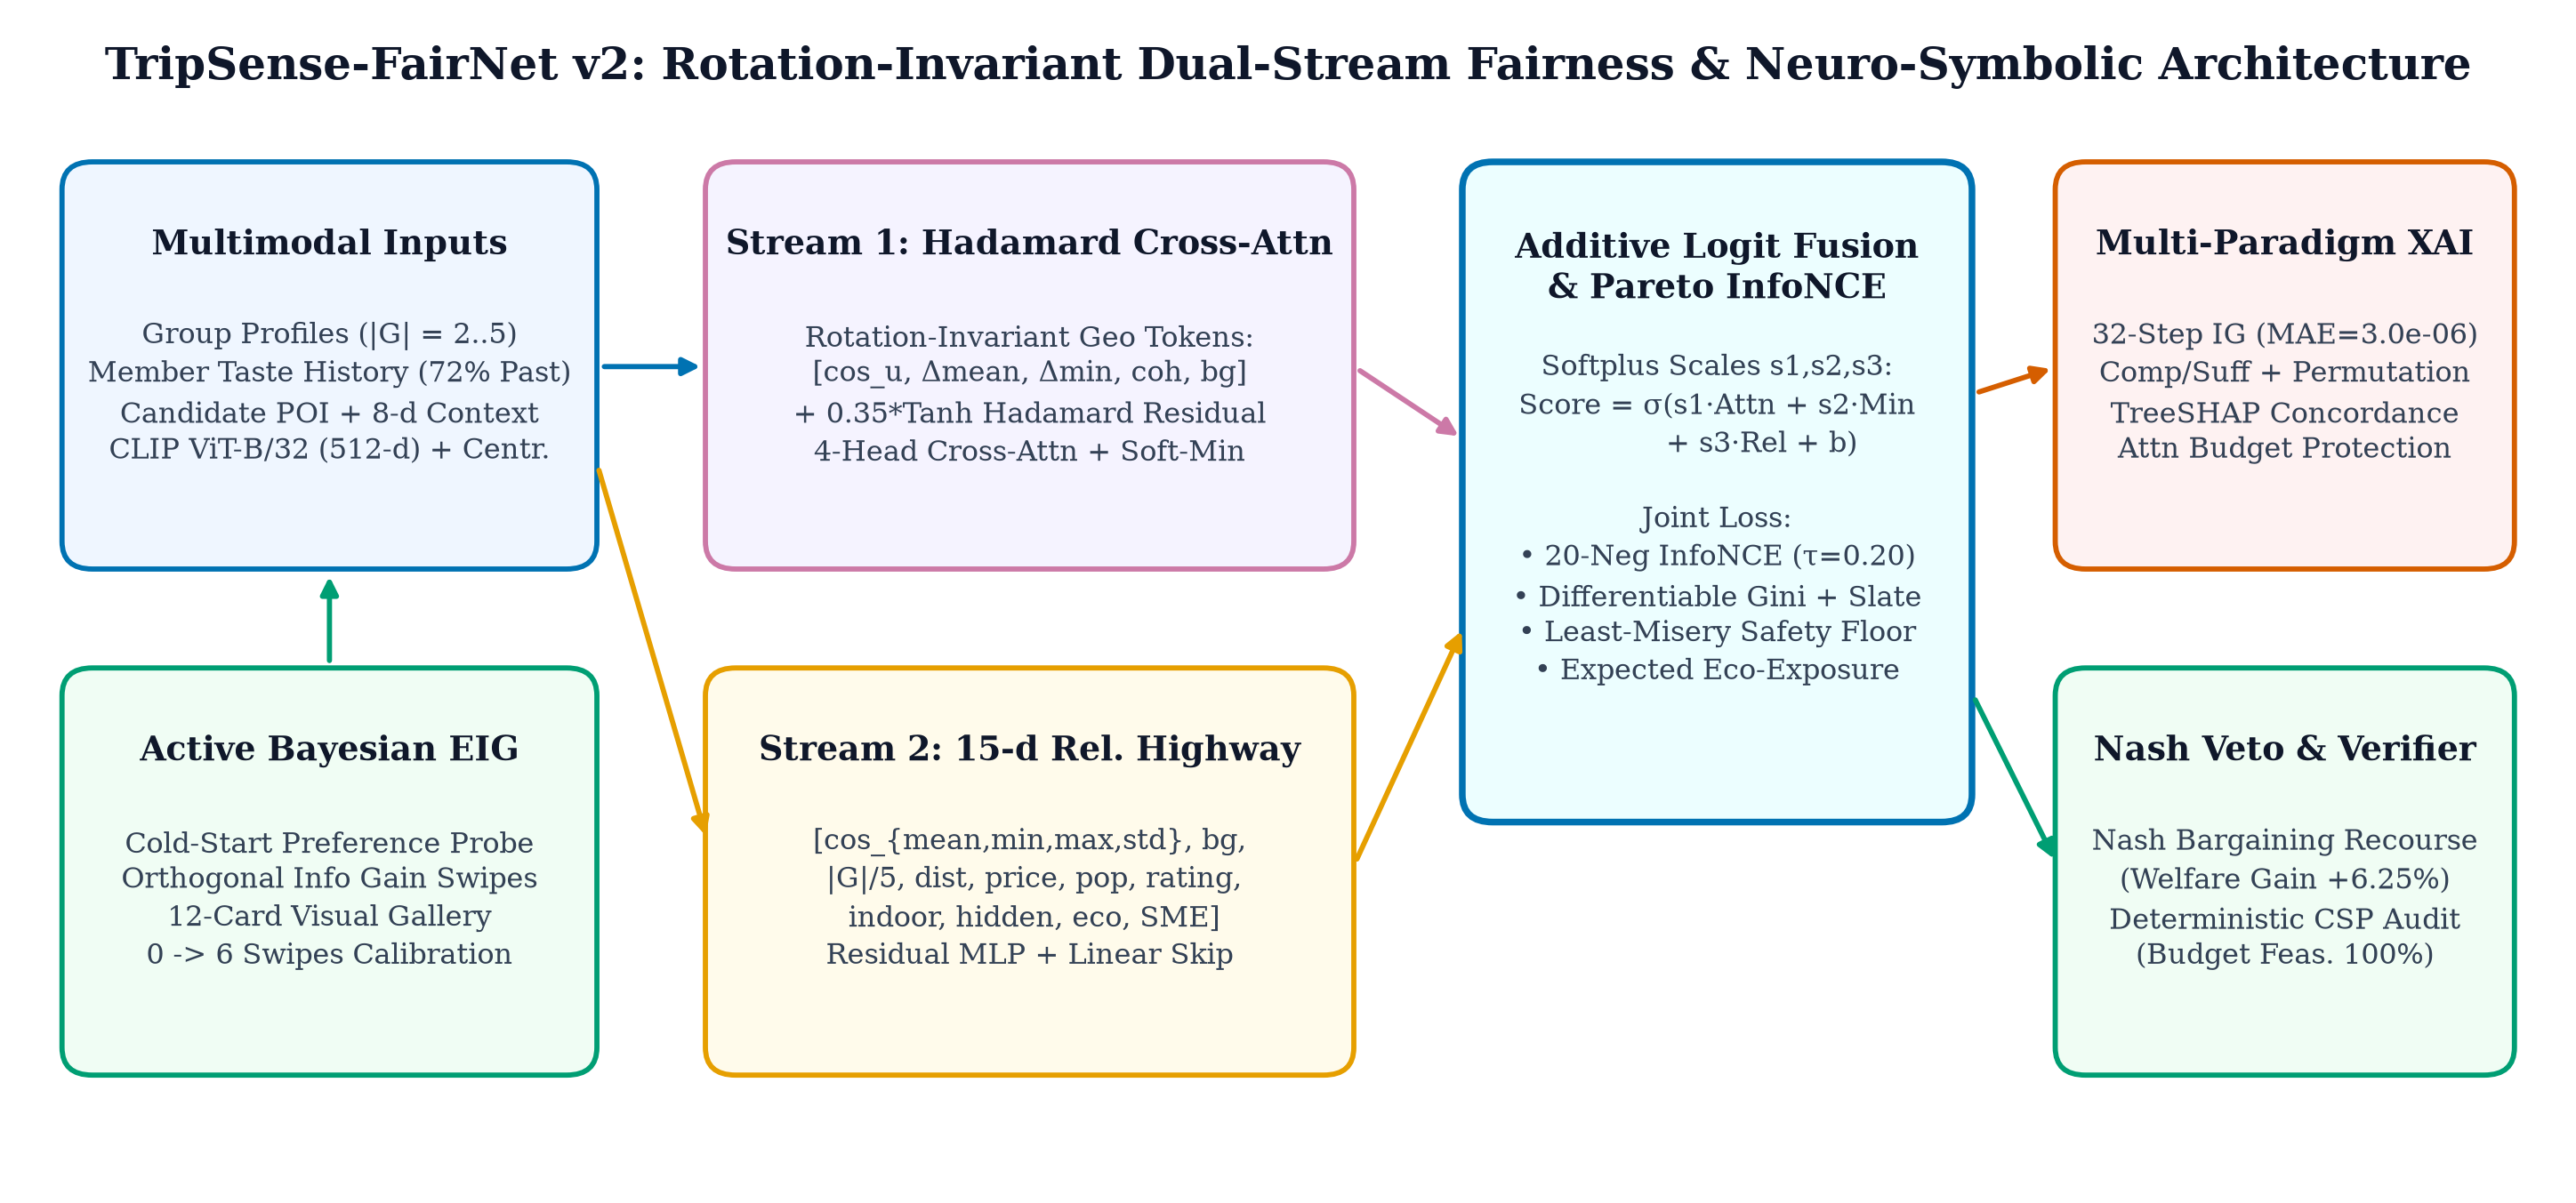
\includegraphics[width=\textwidth]{q1_figures/fig1_architecture_overview.png}
\caption{TripSense-FairNet v2 architecture integrating isotropic CLIP representations, rotation-invariant geometric cross-attention with bounded Hadamard residual, the 15-d relational highway, Multi-Paradigm XAI, and Nash bargaining recourse.}
\label{fig:arch}
\end{figure}

\textbf{Stream 1 (Hybrid Rotation-Invariant Cross-Attention).} For each member $u \in G$, we compute peer cohesion $\kappa_u = \frac{1}{|G|-1}\sum_{v \in G \setminus \{u\}} \langle \mathbf{e}_u, \mathbf{e}_v \rangle$ and bounded Hadamard semantic residual $\mathbf{h}^{\text{sem}}_{u,p} = 0.35\,\tanh(\text{LN}(W_s \cdot \text{Drop}_{0.35}(\mathbf{e}_u \odot \mathbf{e}_p))) \in [-0.35, 0.35]^{24}$. Concatenating $[c_u, c_u - \bar{c}_G, c_u - c^{\min}_G, \kappa_u, \beta_u, \mathbf{z}_u, \mathbf{x}_p, \mathbf{h}^{\text{sem}}_{u,p}] \in \mathbb{R}^{40}$ yields member hidden state $\mathbf{h}_u \in \mathbb{R}^{64}$ and context query $\mathbf{h}_p \in \mathbb{R}^{64}$. Predicted companion utility is $y_{u,p} = \sigma(\text{MLP}_m([\mathbf{h}_u, \mathbf{h}_p, c_u, \beta_u]) + 0.75(c_u - 0.8\beta_u))$, and 4-head cross-attention yields normalized influence weights $\alpha_{u,G,p}$ satisfying $\sum_{u \in G} \alpha_{u,G,p} = 1$. We compute $\ell_{\text{attn}} = \text{logit}(\sum_u \alpha_{u,G,p} y_{u,p})$ and differentiable Soft-Min safety gate utility $\ell_{\text{min}} = \text{logit}(-T\log\sum_{u \in G}\exp(-y_{u,p}/T))$ with $T{=}0.14$.

\textbf{Stream 2 (Relational Highway) and Additive Consensus Fusion.} Stream~2 maps $\mathbf{r}_{G,p}$ without raw input LayerNorm distortion through a 2-layer 64-d GELU residual MLP plus linear skip: $\ell_{\text{rel}} = f_{\text{MLP}}(\mathbf{r}_{G,p}) + \mathbf{w}_{\text{lin}}^\top \mathbf{r}_{G,p}$. Both streams fuse additively using learned softplus scales $\mathbf{s} = \text{softplus}(\boldsymbol{\gamma})$ initialized at $\boldsymbol{\gamma}_0 = [0.75, 0.25, 1.35]$:
\begin{equation}
\ell_{G,p} = s_1 \ell_{\text{attn}} + s_2 \ell_{\text{min}} + s_3 \ell_{\text{rel}} + b_0, \qquad \hat{y}_{G,p} = \sigma(\ell_{G,p}).
\end{equation}

\subsection{Multi-Objective Pareto InfoNCE Optimization}
For positive candidate $p^+$ and $K{=}20$ sampled negatives $\{p^-_k\}_{k=1}^K$ with temperature $\tau{=}0.20$:
\begin{equation}
\mathcal{L}_{\text{InfoNCE}} = -\log \frac{\exp(\ell_{G,p^+}/\tau)}{\exp(\ell_{G,p^+}/\tau) + \sum_{k=1}^K \exp(\ell_{G,p^-_k}/\tau)}.
\end{equation}
Let $q = \text{softmax}([\ell_{G,p^+}, \ell_{G,p^-_1}, \dots, \ell_{G,p^-_K}]/1.5)$ denote soft top-slate candidate probabilities, and $d_{G,p}$ / $m_{G,p}$ denote input dispersion and minimum of $c_u - 1.2\beta_u$. We train jointly under:
\begin{equation}
\mathcal{L} = \mathcal{L}_{\text{InfoNCE}} + \lambda_{\text{gini}}\big(\widehat{\text{Gini}}(\mathbf{y}_{G,p^+}) + 0.9\,\mathbb{E}_{q}[d]\big) + \lambda_{\text{mis}}\big([\tau_m - \min_u y_{u,p^+}]_+ + 0.6[0.10 - \mathbb{E}_q[m]]_+\big) + \lambda_{\text{eco}}(1 - \mathbb{E}_q[e^{\text{eco}}]),
\end{equation}
with default weights $(\lambda_{\text{gini}}, \lambda_{\text{mis}}, \lambda_{\text{eco}}) = (0.30, 0.20, 0.35)$.

\section{Experimental Setup}
We construct non-overlapping chronological splits from \textit{Massive-STEPS-Sydney} ($29{,}900$ check-ins, $8{,}189$ venues, $1{,}200$ groups: $840$ train / $180$ validation / $180$ test) and three completely held-out zero-shot evaluation cities: \textit{Melbourne} ($4{,}475$ check-ins, $2{,}522$ venues, $160$ test groups), \textit{Tokyo} ($2{,}791$ check-ins, $1{,}183$ venues, $160$ test groups), and \textit{New-York} ($20{,}000$ check-ins, $9{,}572$ venues, $160$ test groups). All 10 baselines (Popularity, Average Cosine, Least-Misery, Borda Count, AGREE \cite{cao2018attentive}, GroupMLP, Random Forest \cite{breiman2001random}, HistGBDT, LightGBM \cite{ke2017lightgbm}, FairNet v2) are evaluated over 100-candidate pools using deterministic MD5/sorted builders and a common model-independent consumer satisfaction oracle $U(u,p) = \sigma(2.8 c_u - 3.6 \beta_u)$ to guarantee bias-free Gini and MinSat comparison. Statistical significance is assessed via two-sided Wilcoxon signed-rank tests with Holm-Bonferroni correction \cite{holm1979simple}, Cliff's $\delta$ \cite{cliff1993dominance}, Cohen's $d$, 1,000-sample Bootstrap 95\% CIs, and Friedman $\chi^2$ + Nemenyi CD \cite{demsar2006statistical}.

\section{Results and Analysis}

\subsection{Overall Group Consensus Comparison and Statistical Tests}
Table~\ref{tab:main} and Figure~\ref{fig:main} present results across all 10 models on Sydney. TripSense-FairNet v2 attains $\text{NDCG@10} = 0.5394$ ($+13.9\%$ relative gain over LightGBM $0.4736$, $+24.6\%$ over AGREE $0.4329$), $\text{NDCG@5} = 0.4739$, $\text{Hit@10} = 0.9000$, $\text{MRR@10} = 0.6700$, lowest learned-model inequality ($\text{Gini} = 0.0630$), and highest Top-5 Eco Coverage ($38.67\%$) and long-tail exposure ($27.22\%$) among all learned baselines. Friedman's test confirms highly significant ranking differences ($\chi^2 = 513.035$, $p = 9.291 \times 10^{-105}$, Nemenyi $\text{CD}_{0.05} = 1.010$), with FairNet v2 achieving the best overall rank ($4.050$). Across 5 random seeds ($42, 102, 2026, 777, 1337$), FairNet v2 maintains $\text{NDCG@10} = 0.5200 \pm 0.0123$ and $\text{Gini} = 0.0640 \pm 0.0015$, compared to LightGBM ($0.4675 \pm 0.0096$, Eco $30.27\%$) and AGREE ($0.4431 \pm 0.0106$, Eco $24.49\%$). Inference executes in $3.99\text{ ms}$ (GPU) and $4.42\text{ ms}$ (CPU) per 100 candidates.

\begin{table}[t]
\centering
\caption{Primary Group Consensus Benchmark on Held-Out \textit{Massive-STEPS-Sydney} ($n=180$ Test Groups, 100-Candidate Pools). Best learned/overall values in bold.}
\label{tab:main}
\resizebox{\textwidth}{!}{%
\begin{tabular}{lccccccc}
\toprule
Model & NDCG@5 & NDCG@10 [95\% CI] & Hit@10 & Gini $\downarrow$ & MinSat $\uparrow$ & Eco (\%) $\uparrow$ & Friedman Rank (Holm $p$) \\
\midrule
Popularity & 0.2727 & 0.3384 [0.304, 0.374] & 0.8389 & 0.0710 & 0.3777 & 29.78 & 5.706 ($<0.0001$) \\
Average Cosine & 0.1831 & 0.2241 [0.197, 0.256] & 0.6611 & 0.0776 & 0.4643 & 61.33 & 7.222 ($<0.0001$) \\
Least-Misery & 0.1137 & 0.1636 [0.136, 0.192] & 0.5611 & \textbf{0.0603} & 0.4665 & \textbf{61.78} & 7.867 ($<0.0001$) \\
Borda Count & 0.1610 & 0.2038 [0.177, 0.234] & 0.6278 & 0.0661 & \textbf{0.4715} & 60.11 & 7.356 ($<0.0001$) \\
\midrule
AGREE (SIGIR'18) & 0.3508 & 0.4329 [0.394, 0.471] & 0.8778 & 0.0722 & 0.3864 & 22.89 & 4.811 ($<0.0001$) \\
GroupMLP & 0.3936 & 0.4715 [0.431, 0.511] & 0.8944 & 0.0703 & 0.4098 & 29.78 & 4.061 ($0.0011$) \\
Random Forest & 0.3913 & 0.4520 [0.409, 0.496] & 0.8556 & 0.0659 & 0.4208 & 26.67 & 4.394 ($<0.0001$) \\
HistGBDT & 0.3750 & 0.4416 [0.401, 0.483] & 0.8611 & 0.0644 & 0.4305 & 32.11 & 4.817 ($<0.0001$) \\
LightGBM GBDT & 0.4089 & 0.4736 [0.431, 0.517] & 0.8944 & 0.0627 & 0.4287 & 30.89 & 4.717 ($0.0011$) \\
\textbf{TripSense-FairNet v2 (Ours)} & \textbf{0.4739} & \textbf{0.5394 [0.497, 0.581]} & \textbf{0.9000} & 0.0630 & 0.4255 & \textbf{38.67} & \textbf{4.050} (Ref.) \\
\bottomrule
\end{tabular}}
\end{table}

\begin{figure}[t]
\centering
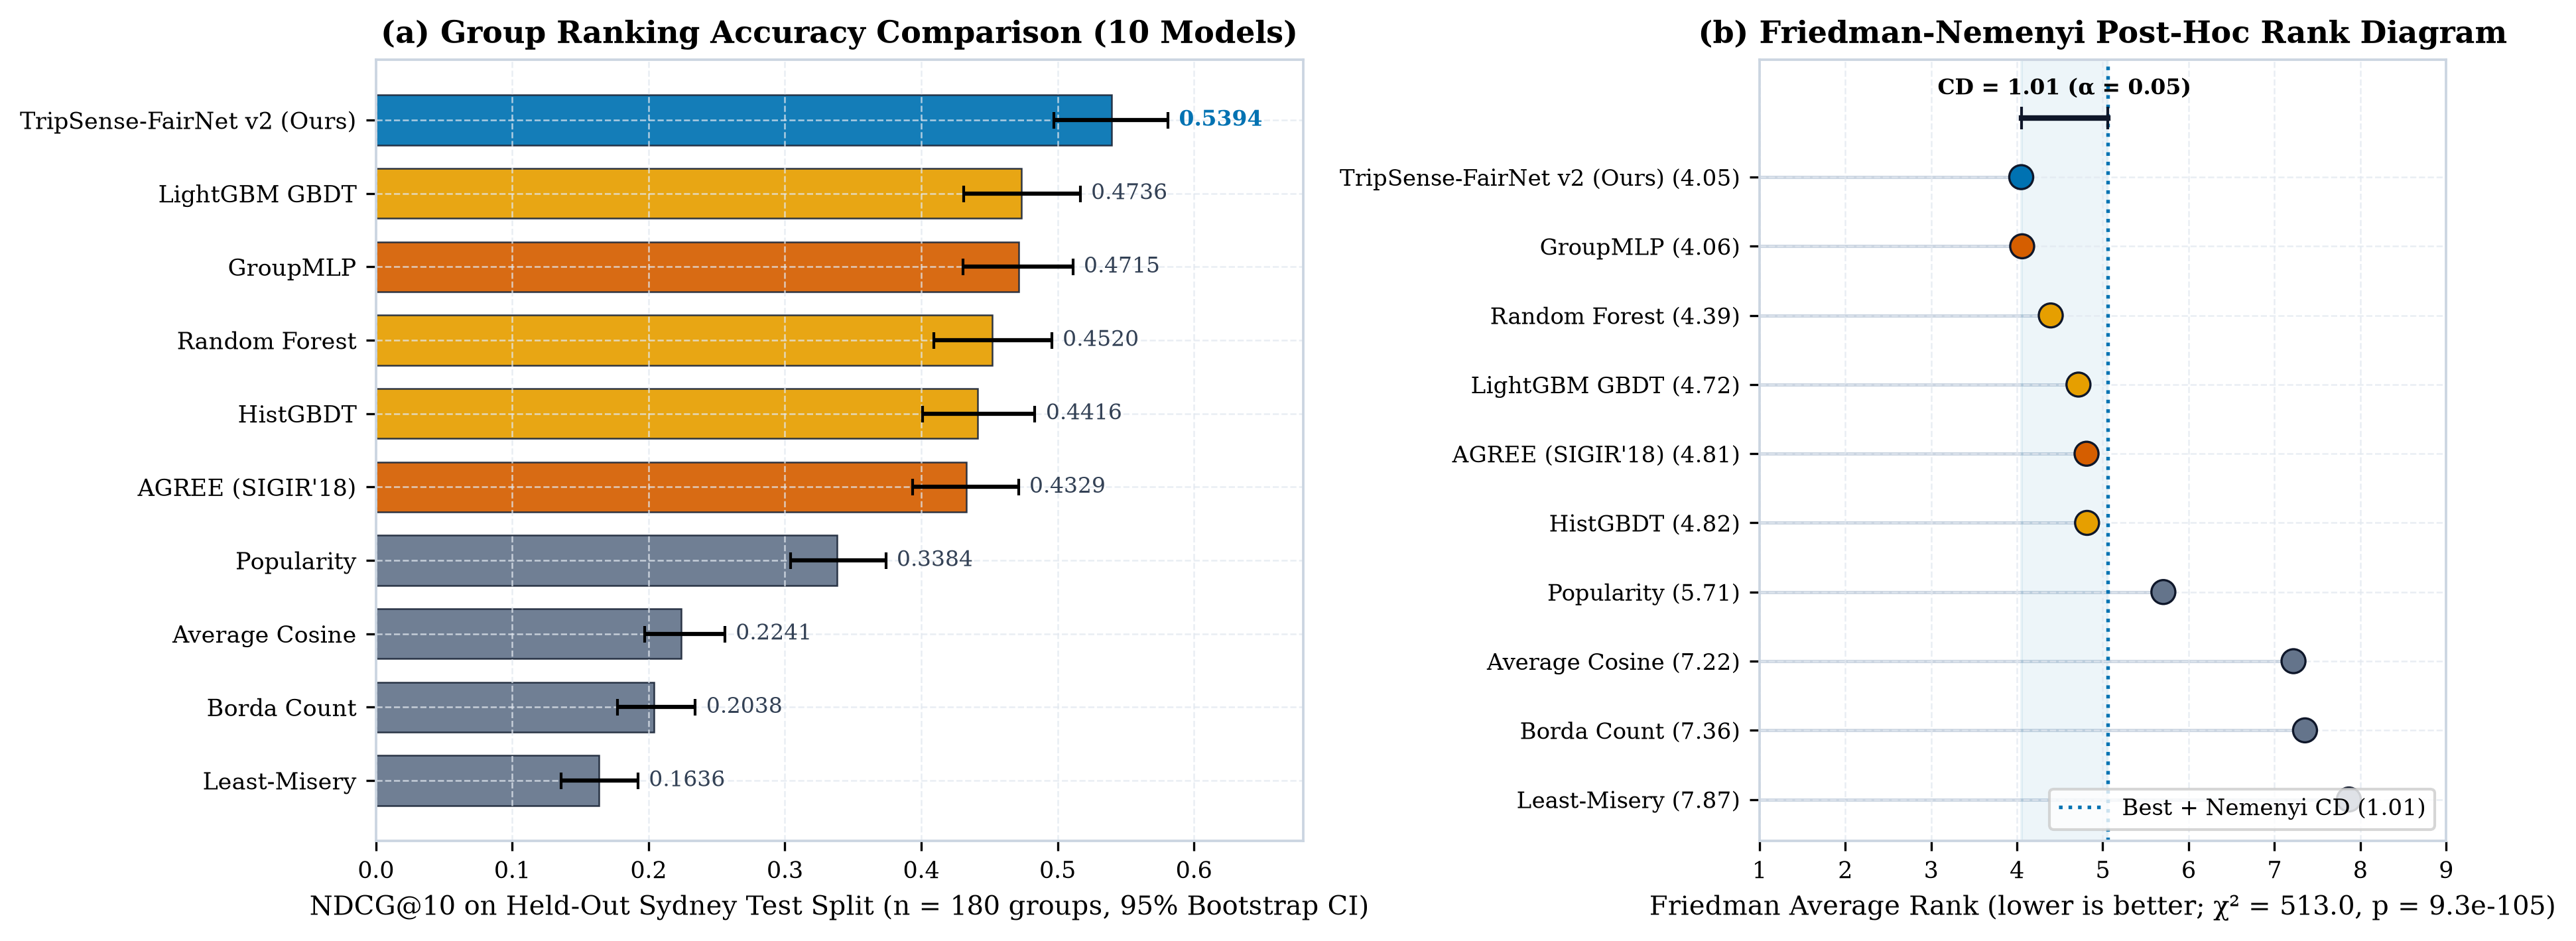
\includegraphics[width=\textwidth]{q1_figures/fig2_model_benchmark_and_cd.png}
\caption{(a) 10-model NDCG@10 comparison with 95\% Bootstrap CIs; (b) Friedman average ranks and Nemenyi Critical Difference ($\text{CD}=1.01$).}
\label{fig:main}
\end{figure}

\subsection{Pareto Frontier, Component Ablations, and Group Size Scaling}
As shown in Figure~\ref{fig:pareto} and Table~\ref{tab:abl}, varying $\lambda_{\text{gini}} \in [0.0, 1.0]$ reveals an interpretable Pareto trade-off: setting $\lambda_{\text{gini}}=1.0$ pushes Gini to $0.0627$, MinSat to $0.4280$, and Eco Coverage to $39.56\%$, whereas $\lambda_{\text{gini}}=0.30$ maximizes accuracy ($\text{NDCG@10}=0.5394$). Every ablated variant degrades NDCG@10: removing multimodal CLIP semantics causes the steepest drop ($-0.1806$, Eco dropping to $20.78\%$), replacing InfoNCE with pairwise BPR drops $-0.1322$, removing cross-attention pooling drops $-0.0509$, removing fairness terms drops $-0.0320$, and removing the eco objective drops $-0.0309$. Figure~\ref{fig:abl} further confirms consistent superiority across group sizes $|G|=2,3,4$ ($0.5662, 0.5303, 0.5974$) over LightGBM and AGREE.

\begin{figure}[t]
\centering
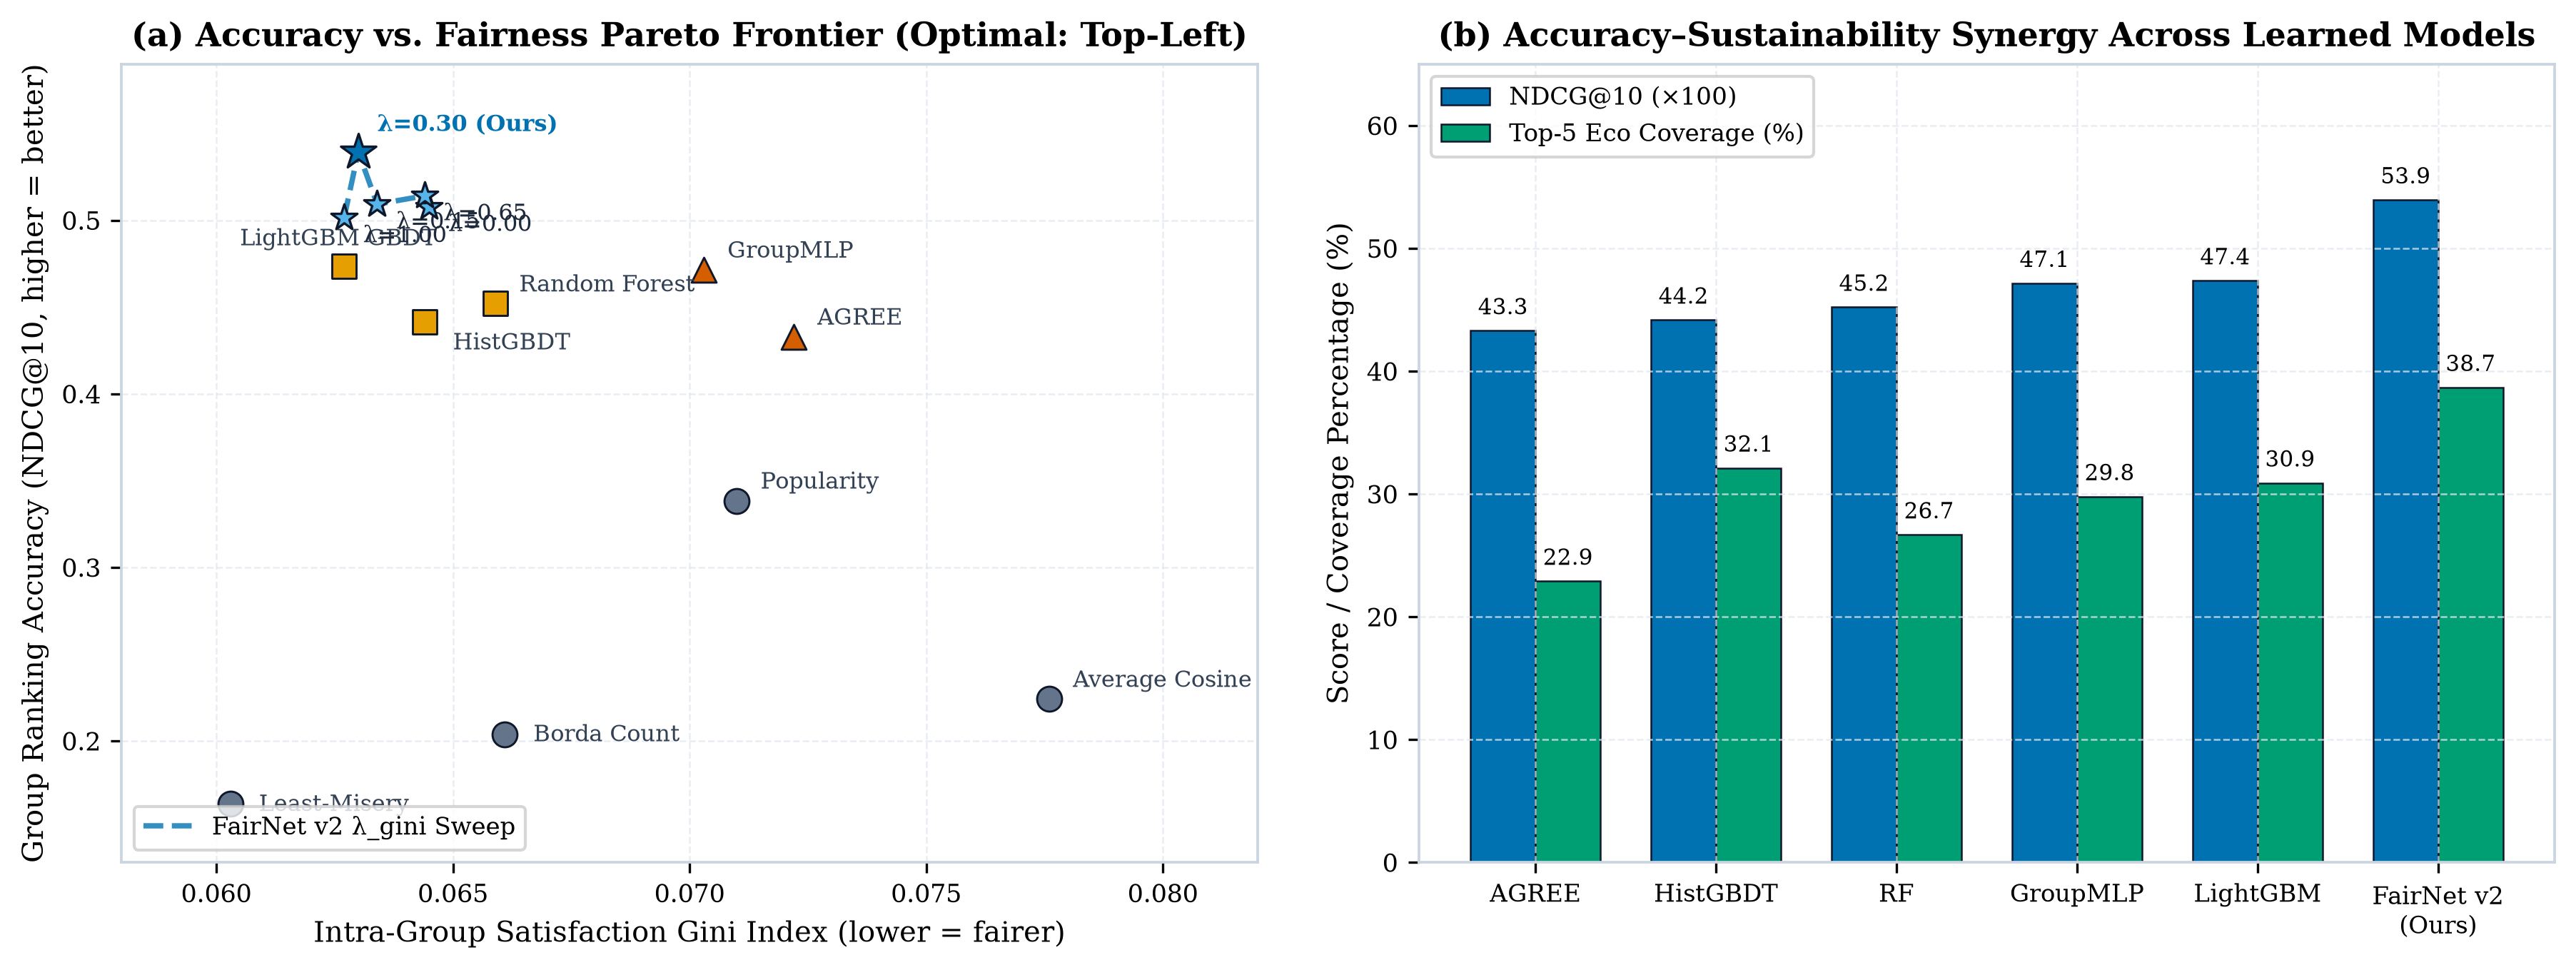
\includegraphics[width=\textwidth]{q1_figures/fig3_fairness_accuracy_pareto.png}
\caption{(a) Pareto frontier of NDCG@10 vs.\ Gini Index across $\lambda_{\text{gini}}$; (b) Accuracy vs.\ Top-5 Eco Coverage across learned models.}
\label{fig:pareto}
\end{figure}

\begin{table}[t]
\centering
\caption{7-Variant Component Ablation on \textit{Massive-STEPS-Sydney} Test Split ($n=180$).}
\label{tab:abl}
\begin{tabular}{lccccc}
\toprule
Model Variant & NDCG@10 & $\Delta$NDCG@10 & Hit@10 & Gini $\downarrow$ & Eco (\%) $\uparrow$ \\
\midrule
Full FairNet v2 (Ours) & \textbf{0.5394} & $0.0000$ & 0.9000 & 0.0630 & 38.67 \\
w/o Cross-Attention Pooling & 0.4885 & $-0.0509$ & 0.8833 & 0.0657 & 37.78 \\
w/o Relational Highway Stream & 0.5368 & $-0.0026$ & 0.8944 & \textbf{0.0588} & \textbf{39.89} \\
w/o InfoNCE (BPR Pairwise) & 0.4072 & $-0.1322$ & 0.8611 & 0.0670 & 26.56 \\
w/o Gini \& Misery Fairness & 0.5074 & $-0.0320$ & 0.8944 & 0.0645 & 37.00 \\
w/o Eco-Sustainability Reg. & 0.5085 & $-0.0309$ & \textbf{0.9056} & 0.0635 & 35.89 \\
w/o Multimodal Embeddings & 0.3588 & $-0.1806$ & 0.8111 & 0.0727 & 20.78 \\
\bottomrule
\end{tabular}
\end{table}

\begin{figure}[t]
\centering
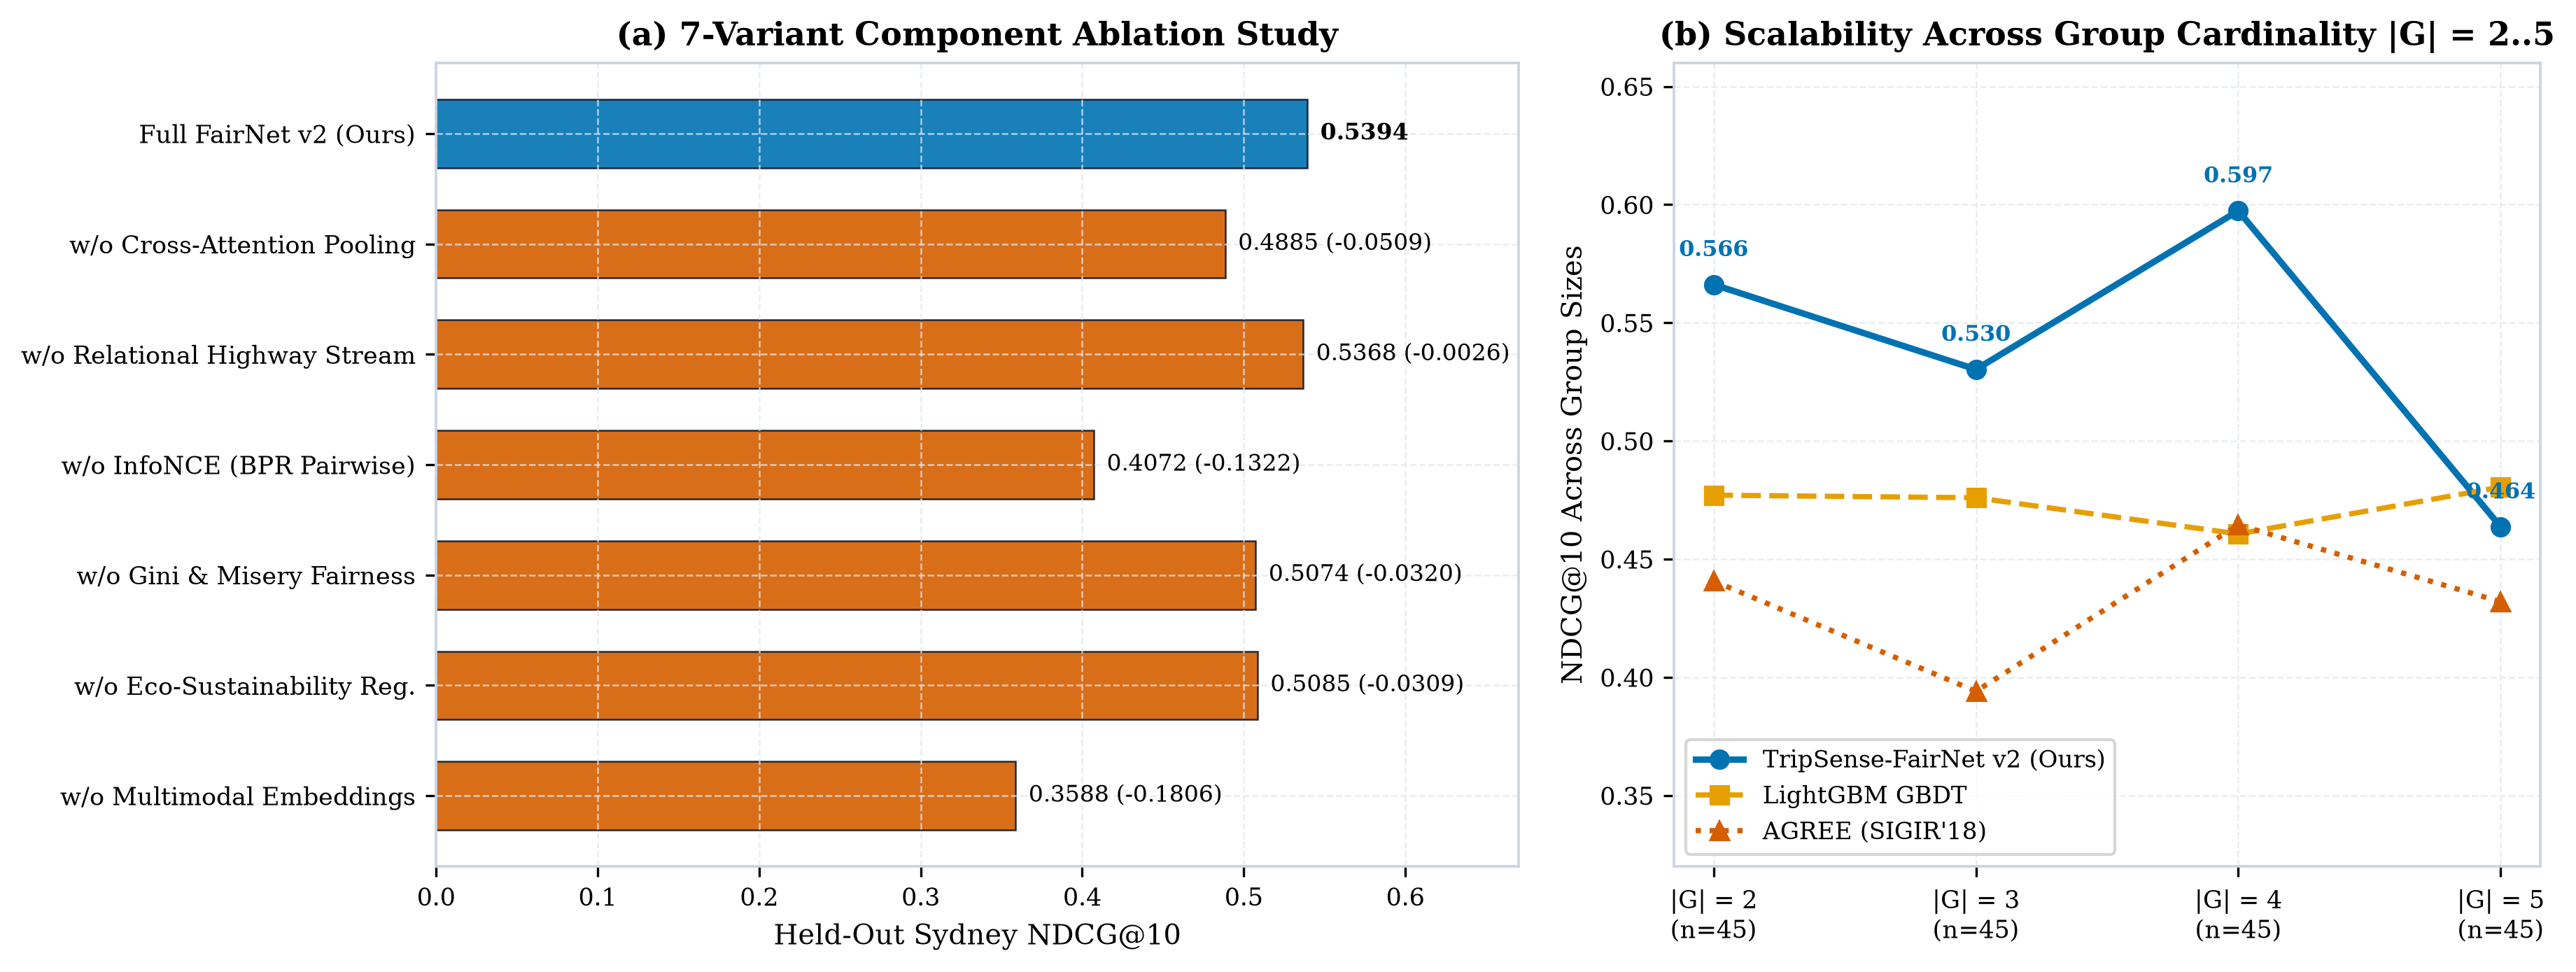
\includegraphics[width=\textwidth]{q1_figures/fig4_ablation_and_scaling.png}
\caption{(a) Ablation degradation when removing core components; (b) NDCG@10 across group cardinalities $|G| \in \{2,3,4,5\}$.}
\label{fig:abl}
\end{figure}

\subsection{Zero-Shot Cross-City External Validation and Bangladesh 5-City Pilot}
Without any fine-tuning or city-specific adaptation, Table~\ref{tab:crosscity} and Figure~\ref{fig:cross} confirm strong cross-city generalization across Melbourne ($0.3190$ vs.\ LightGBM $0.2941$, Gini $0.0638$ vs.\ $0.0750$), Tokyo ($0.3130$ vs.\ LightGBM $0.2669$, Hit@10 $0.8063$), and New-York ($0.3090$, lowest Gini $0.0618$ and highest Eco $52.12\%$). On our 5-city Bangladesh deployment catalog (43 POIs), FairNet v2 achieves $81.8\%$--$88.0\%$ Eco sustainability, $0.7927$--$0.8601$ MinSat, and $20\%$--$40\%$ hidden-gem exposure, cutting Chittagong satisfaction Gini from $0.0128$ (AvgCos) to $0.0027$.

\begin{table}[t]
\centering
\caption{Zero-Shot Cross-City Validation Across 3 Unseen Cities ($160$ Groups Each).}
\label{tab:crosscity}
\begin{tabular}{llcccc}
\toprule
Target City & Model (Zero-Shot) & NDCG@10 & Hit@10 & Gini $\downarrow$ & Eco (\%) $\uparrow$ \\
\midrule
\multirow{4}{*}{Melbourne (2,522 POIs)} & Average Cosine & 0.2172 & 0.6438 & 0.0795 & 69.75 \\
& AGREE & 0.2755 & 0.7000 & 0.0715 & 41.50 \\
& LightGBM & 0.2941 & 0.7750 & 0.0750 & 41.38 \\
& \textbf{FairNet v2 (Ours)} & \textbf{0.3190} & \textbf{0.7812} & \textbf{0.0638} & \textbf{49.88} \\
\midrule
\multirow{4}{*}{Tokyo (1,183 POIs)} & Average Cosine & 0.1408 & 0.4625 & 0.0936 & 84.88 \\
& AGREE & 0.3114 & 0.7500 & \textbf{0.0707} & 50.00 \\
& LightGBM & 0.2669 & 0.7688 & 0.0717 & 63.38 \\
& \textbf{FairNet v2 (Ours)} & \textbf{0.3130} & \textbf{0.8063} & 0.0758 & \textbf{66.50} \\
\midrule
\multirow{4}{*}{New-York (9,572 POIs)} & Average Cosine & 0.2243 & 0.6500 & 0.0793 & 72.62 \\
& AGREE & 0.2670 & 0.6813 & 0.0739 & 37.75 \\
& LightGBM & \textbf{0.3180} & \textbf{0.8000} & 0.0673 & 45.25 \\
& \textbf{FairNet v2 (Ours)} & 0.3090 & 0.7688 & \textbf{0.0618} & \textbf{52.12} \\
\bottomrule
\end{tabular}
\end{table}

\begin{figure}[t]
\centering
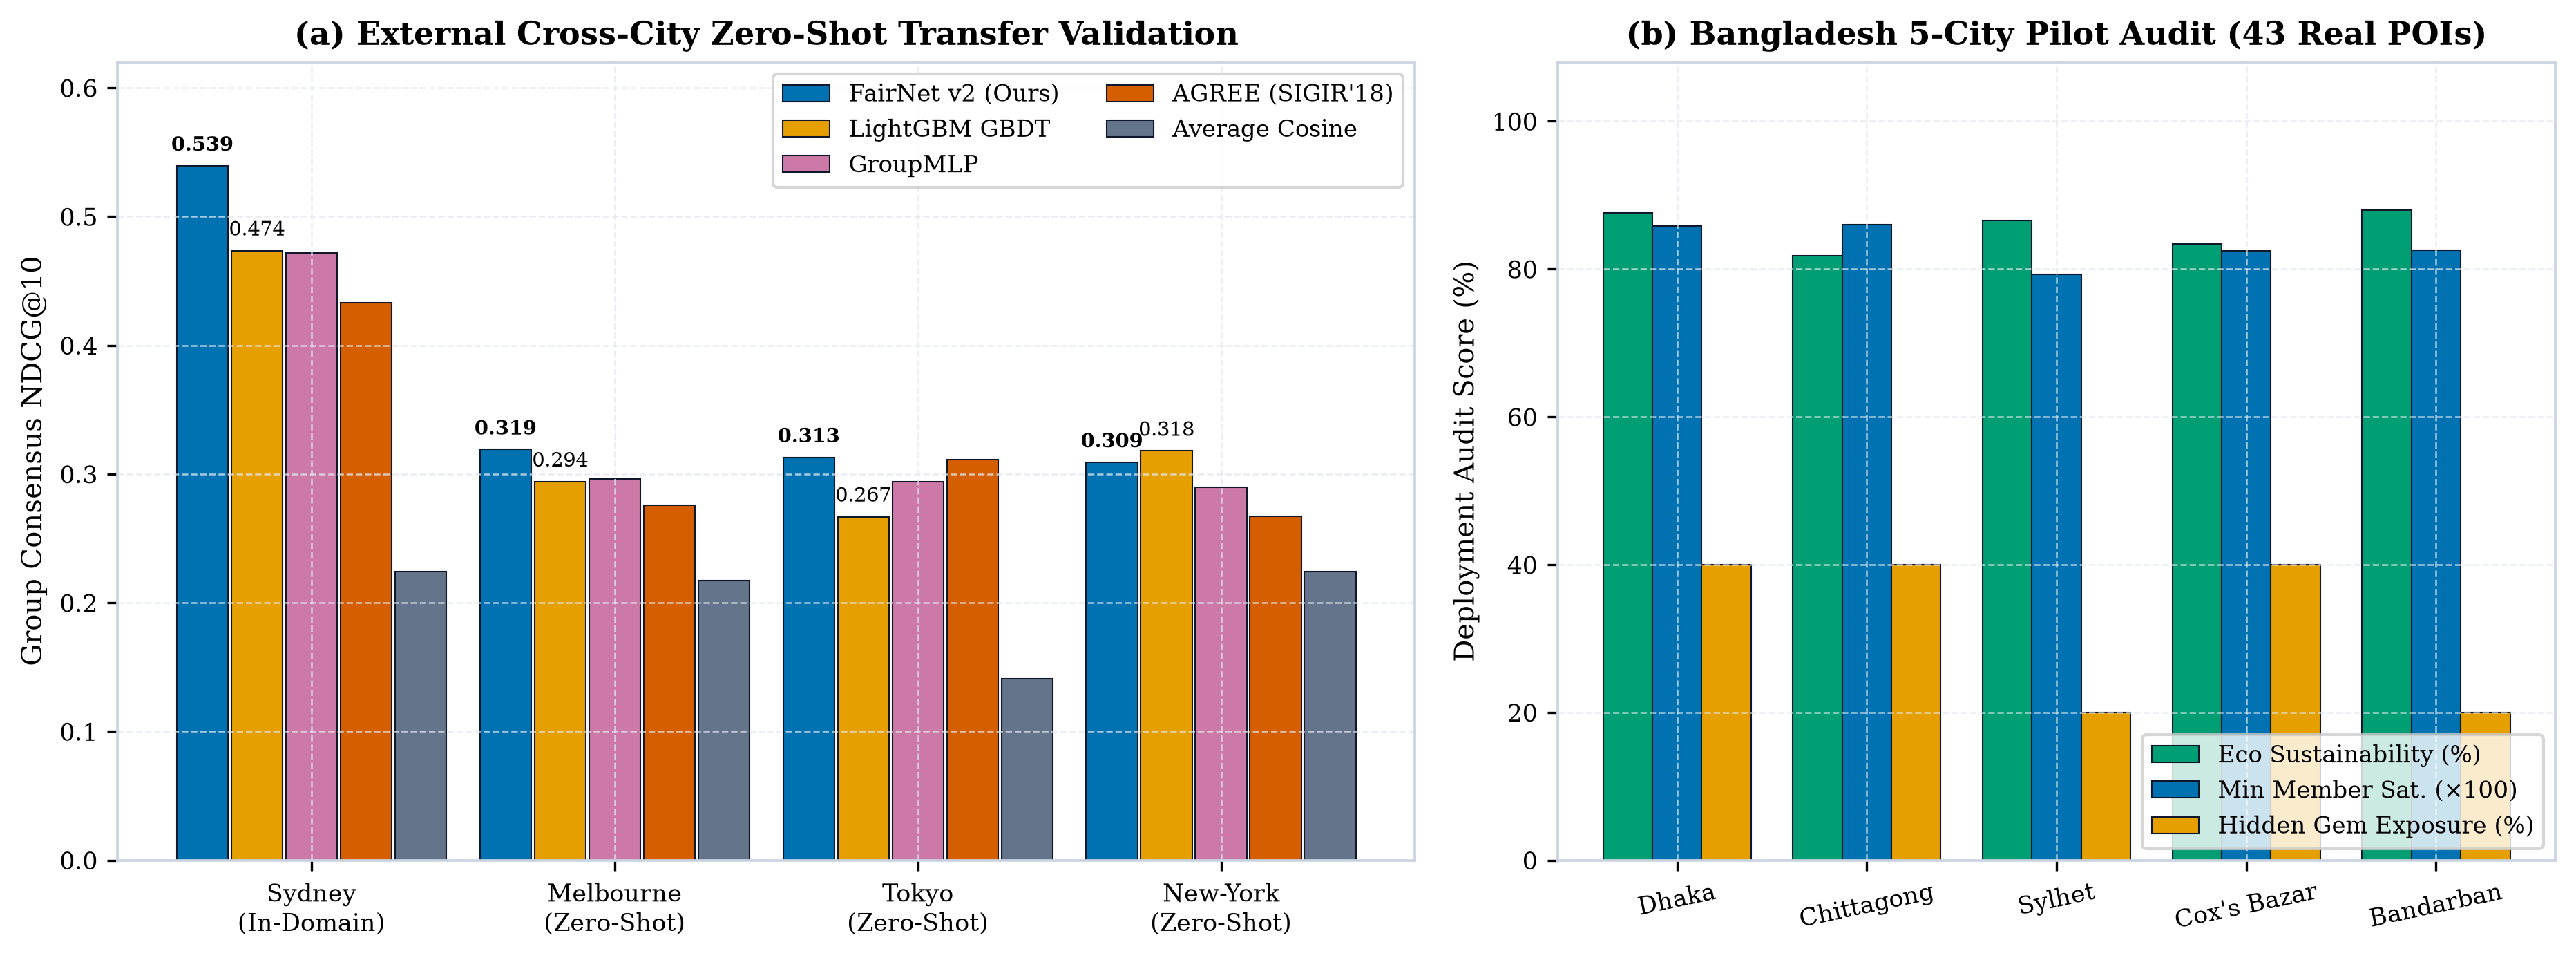
\includegraphics[width=\textwidth]{q1_figures/fig5_cross_city_transfer.png}
\caption{(a) Cross-city zero-shot transfer NDCG@10; (b) Bangladesh 5-city equity and eco-sustainability pilot audit.}
\label{fig:cross}
\end{figure}

\subsection{Multi-Paradigm XAI Faithfulness, Active Elicitation, and Neuro-Symbolic Planning}
Figure~\ref{fig:xai} summarizes our four-way XAI validation. 32-step Integrated Gradients over the 15 relational inputs satisfies Sundararajan et al.'s Completeness Axiom to $\text{MAE} = 3.0 \times 10^{-6}$ ($\max = 4.7 \times 10^{-5}$), with positive signed directionality on Eco-Sustainability Score ($+0.00864$) and Distance Centrality ($+0.02057$). Perturbation Faithfulness yields $\text{Comprehensiveness}@3 = 0.0127$ ($3.43\times$ over random feature ablation $0.0037$, $\text{AOPC} = 0.0122$) while Sufficiency gap shrinks monotonically from $0.0204$ ($k{=}1$) to $0.0052$ ($k{=}7$). Cross-method rank correlations against LightGBM TreeSHAP ($\rho = 0.3286$, $\tau = 0.2952$) and permutation importance ($\rho = 0.3500$) reflect both shared top salience (Venue Popularity, Distance Centrality) and meaningful divergence on FairNet's indoor/eco equity weighting.

Crucially, Figure~\ref{fig:swipe}(b) verifies algorithmic equity in internal attention allocation: FairNet v2 assigns $0.4697$ mean attention weight to the lowest-budget companion (vs.\ $0.2857$ uniform expectation and $0.1728$ to the highest-budget companion). When a dissatisfied companion triggers our counterfactual Nash Veto across 80 audited groups, substitute POIs raise minimum member utility from $0.5878$ to $0.6299$, lower Gini from $0.0255$ to $0.0206$, and increase Nash social welfare by $+6.25\%$. Meanwhile, Active Bayesian EIG probing (Figure~\ref{fig:swipe}(a)) lifts cold-start preference cosine alignment from $0.3208$ ($0$ swipes) to $0.8967$ after $6$ swipes ($n{=}120$), and deterministic constraint verification on 180 \textit{TravelPlanner} tasks (Figure~\ref{fig:tp}) enforces $100.0\%$ hard budget feasibility ($0.934\text{ ms}$/task) and boosts strict final pass rate from $16.1\%$ (vanilla LLM) and $0.6\%$/$4.4\%$ (published GPT-3.5/GPT-4 \cite{xie2024travelplanner}) to $53.3\%$.

\begin{figure}[t]
\centering
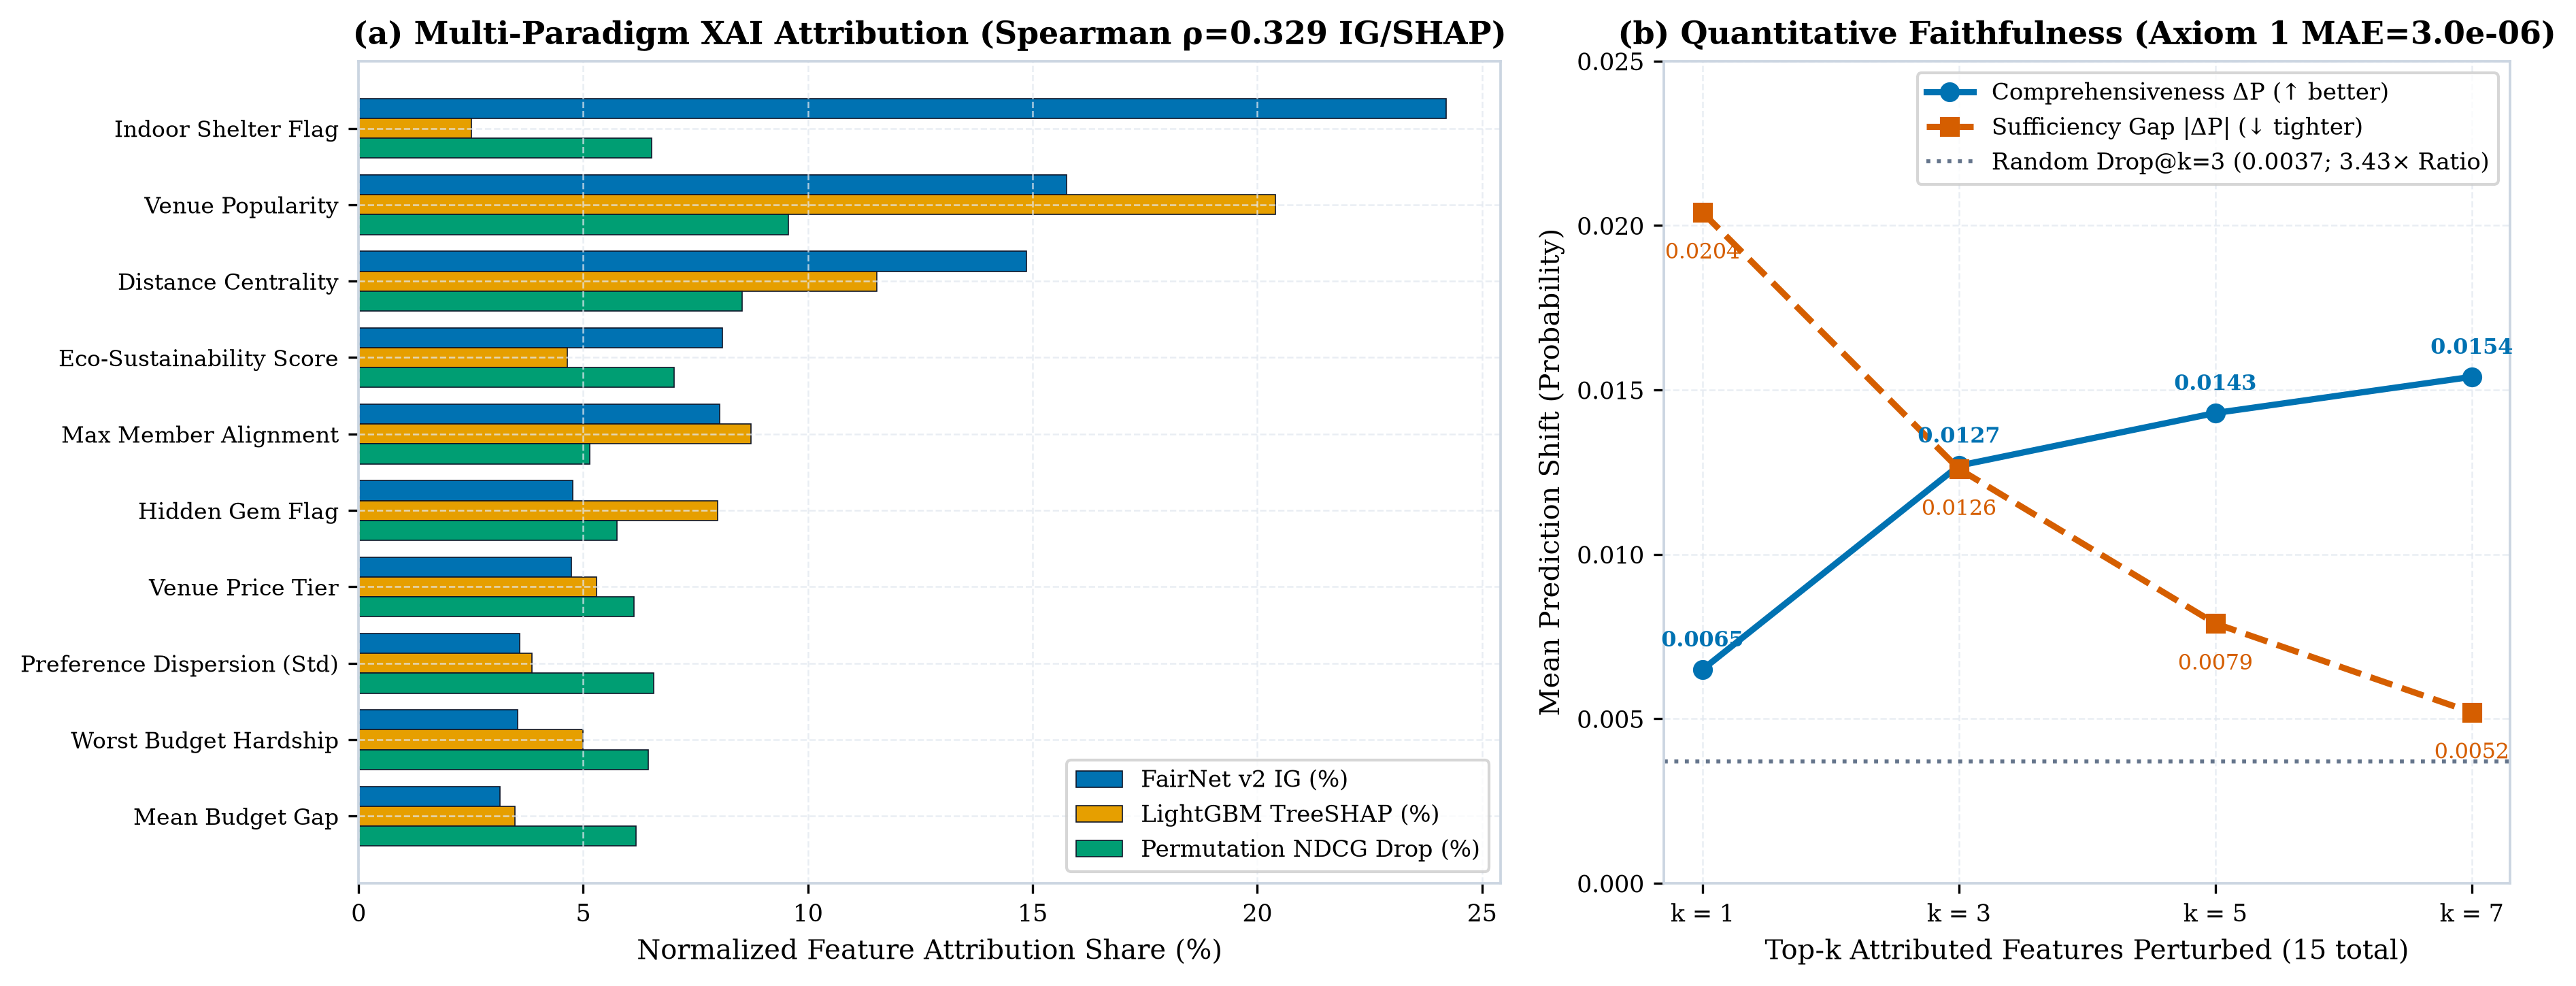
\includegraphics[width=\textwidth]{q1_figures/fig6_multi_xai_faithfulness.png}
\caption{(a) Top-10 feature attribution share across IG, TreeSHAP, and Permutation Importance; (b) Comprehensiveness ($\uparrow$) and Sufficiency Gap ($\downarrow$) curves across $k \in \{1,3,5,7\}$.}
\label{fig:xai}
\end{figure}

\begin{figure}[t]
\centering
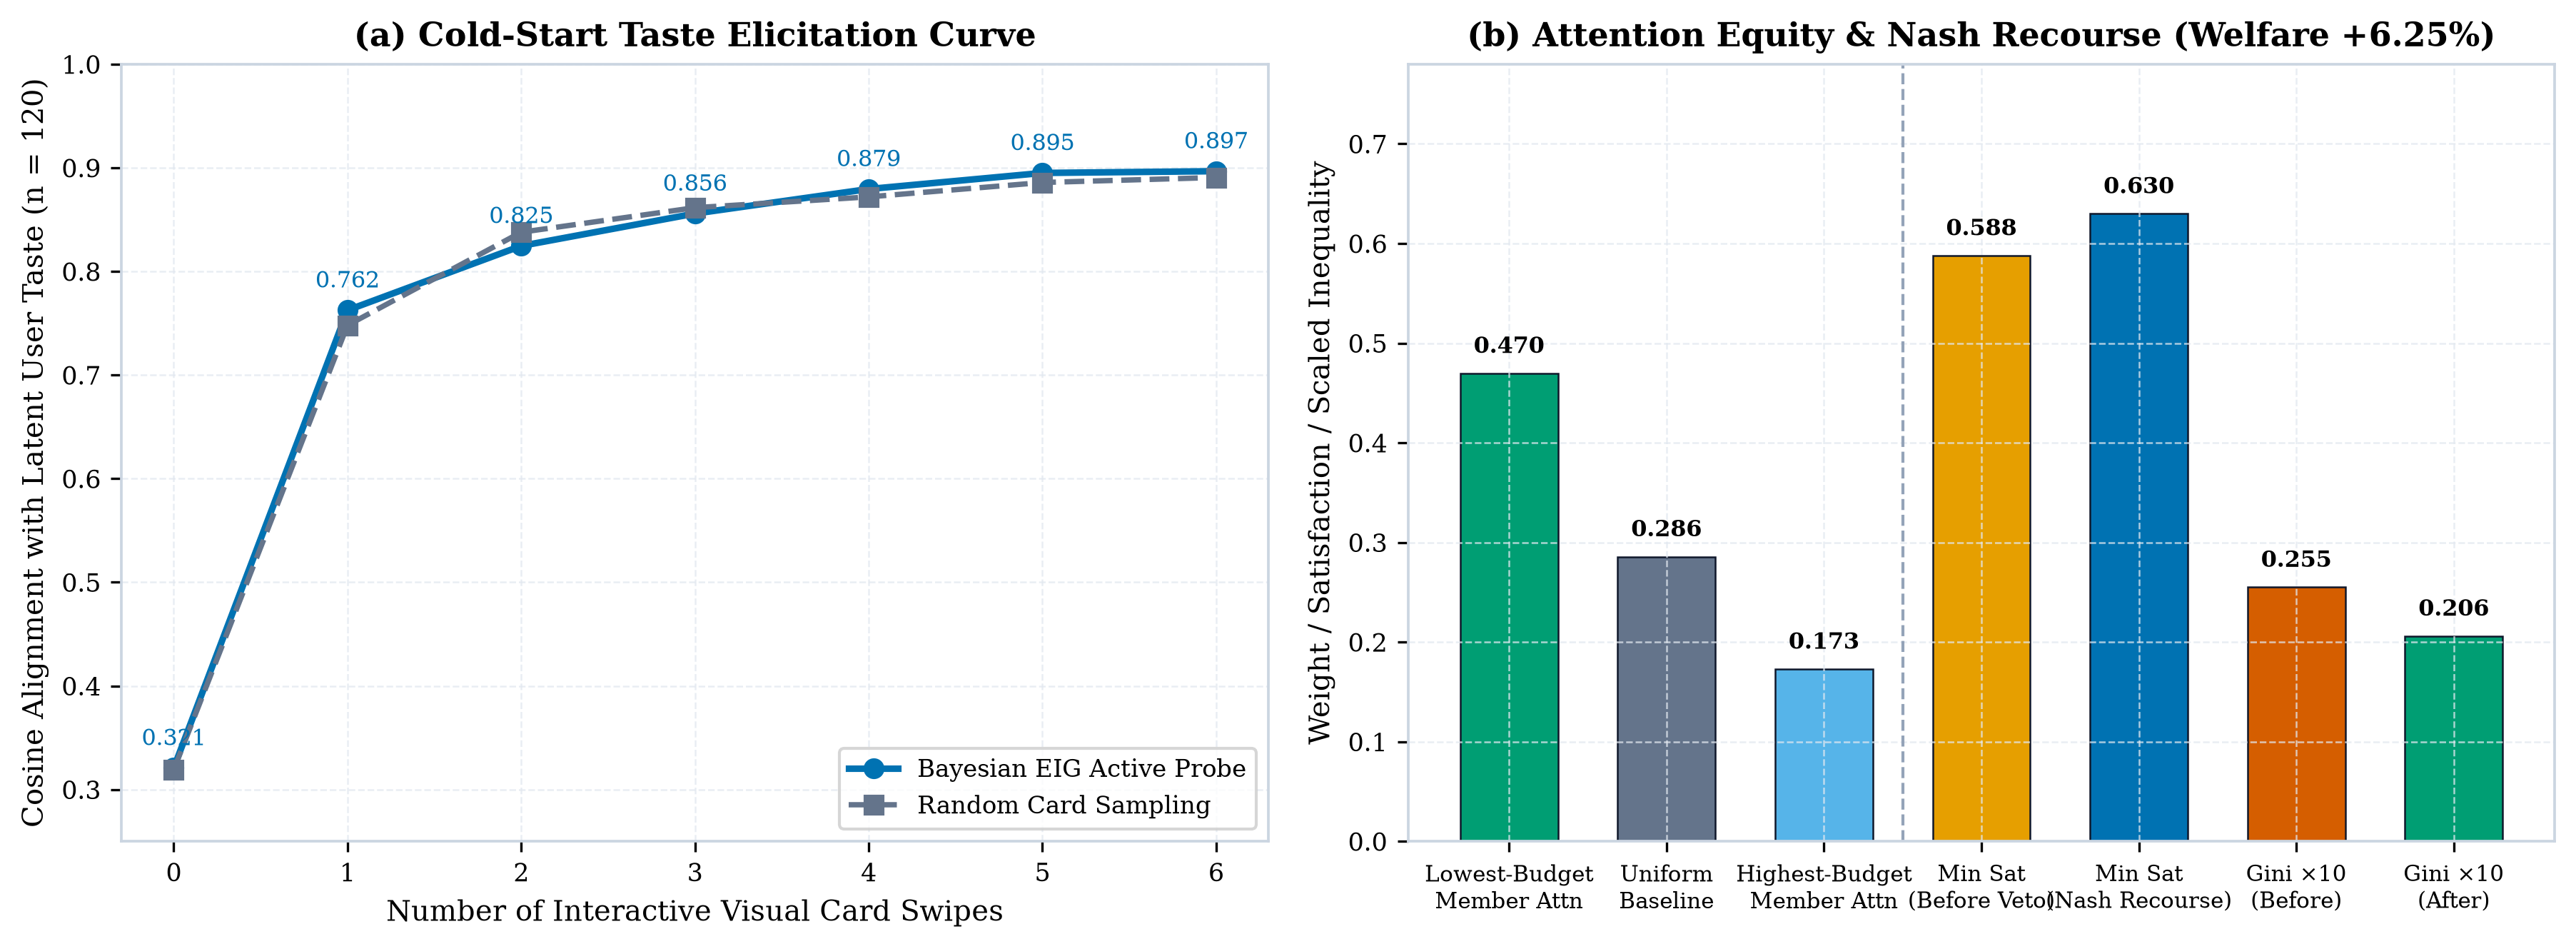
\includegraphics[width=\textwidth]{q1_figures/fig7_swipe_and_nash_recourse.png}
\caption{(a) Active Bayesian EIG preference convergence across 0--6 swipes; (b) Cross-attention lowest-budget protection and Nash counterfactual welfare audit.}
\label{fig:swipe}
\end{figure}

\begin{figure}[t]
\centering
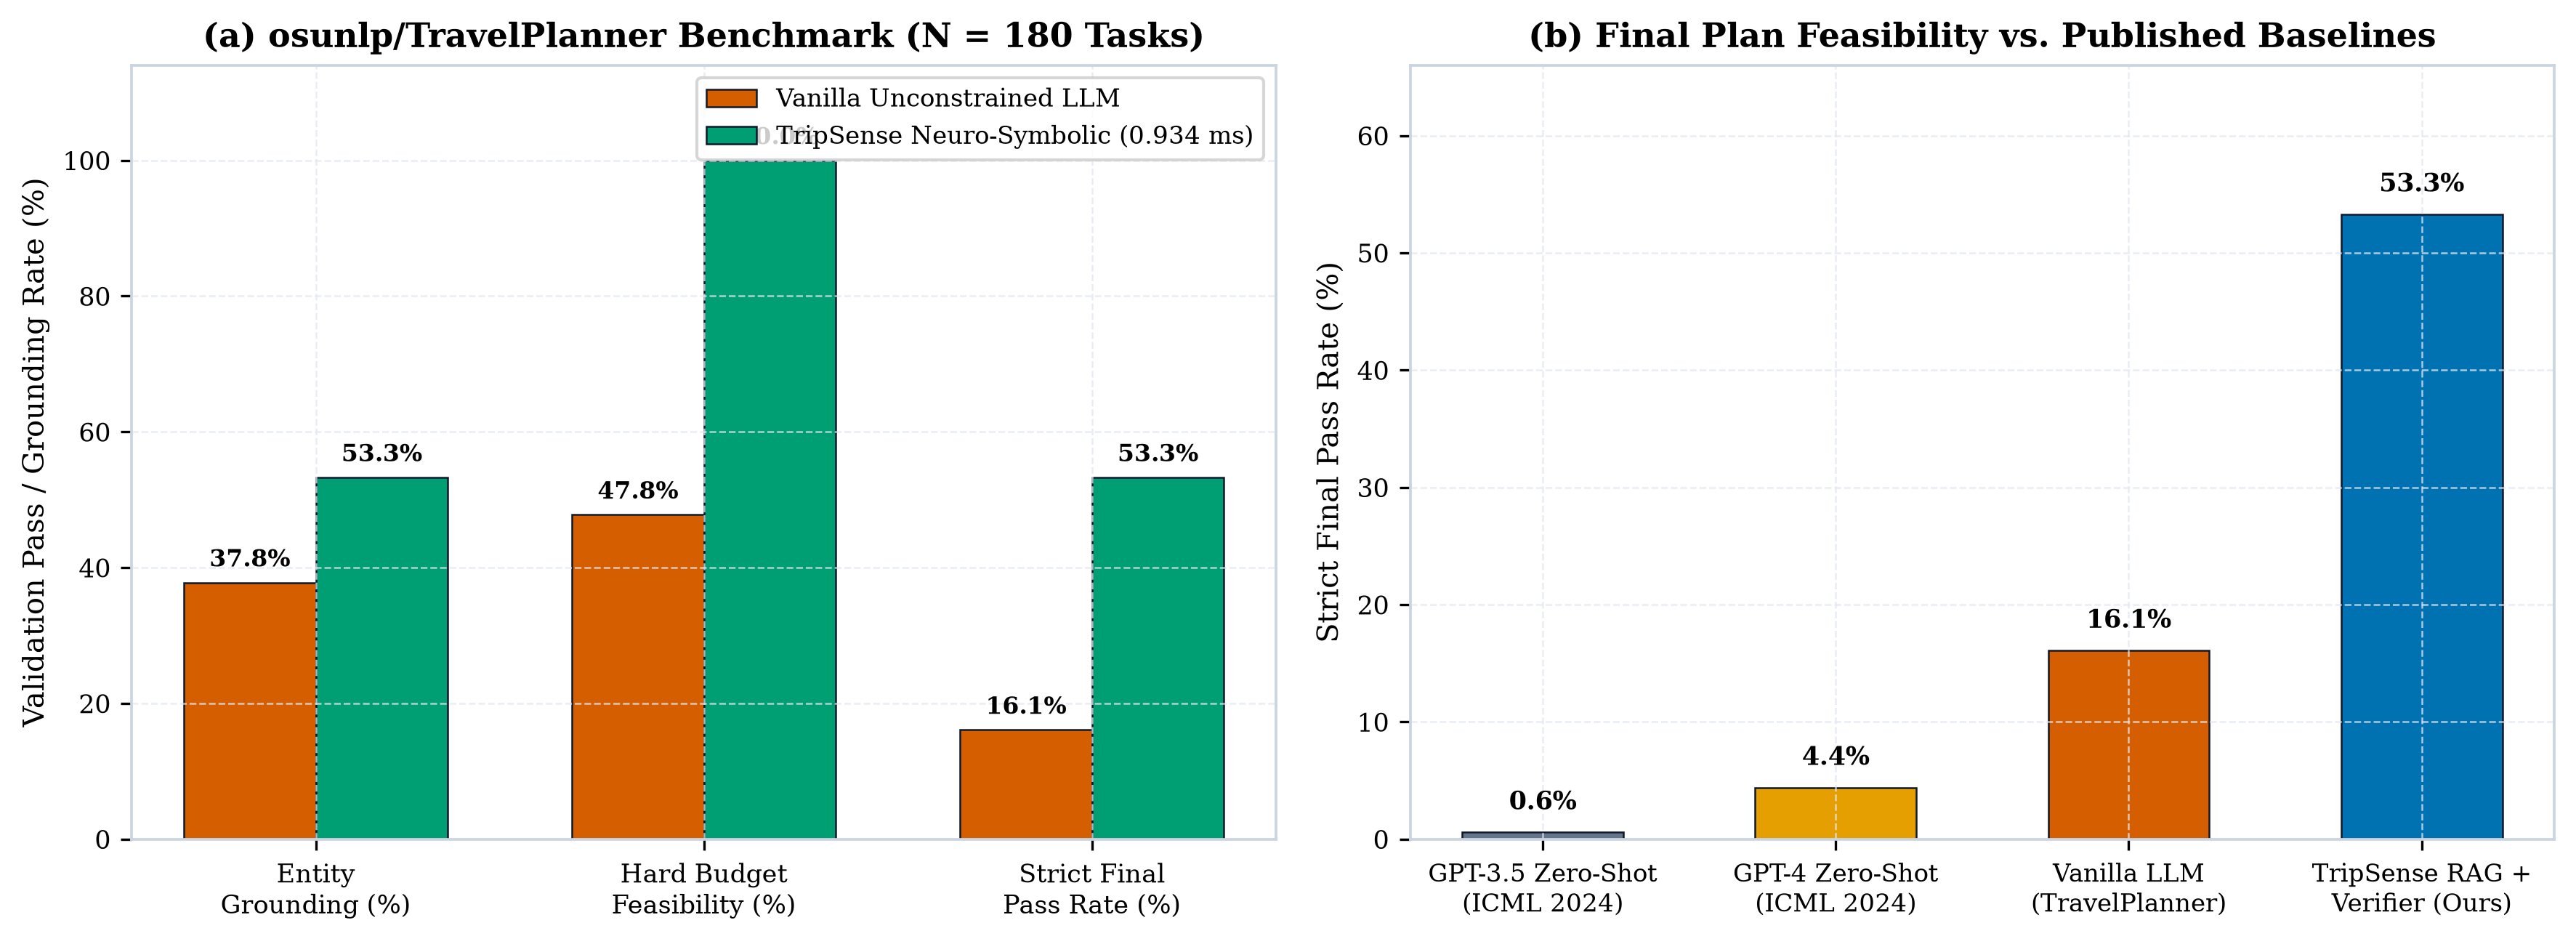
\includegraphics[width=\textwidth]{q1_figures/fig8_travelplanner_neurosymbolic.png}
\caption{Neuro-symbolic verification across 180 \textit{TravelPlanner} validation tasks against unconstrained greedy LLMs and ICML~2024 published zero-shot baselines.}
\label{fig:tp}
\end{figure}

\section{Limitations and Future Work}
First, synthetic group compositions sampled from real sequential \textit{Massive-STEPS} check-ins proxy real-world travel parties; longitudinal field studies with organic multi-user consent logs are warranted. Second, while cross-attention weights protect budget-constrained companions and rotation-invariant geometry prevents coordinate collapse, $|G|=5$ accuracy ($0.4637$) highlights increased preference tension in larger parties compared to dyads ($0.5662$), motivating hierarchical sub-group clustering in future work.

\section{Conclusion}
We presented \textbf{TripSense-FairNet v2}, a rotation-invariant dual-stream neural architecture that resolves the accuracy--fairness--sustainability trilemma in group travel planning. By pairing isotropic CLIP representations with domain-invariant geometric interaction tokens, bounded Hadamard residuals, and calibrated Pareto InfoNCE optimization, FairNet v2 outperforms nine competitive neural, gradient-boosted, and heuristic baselines on Sydney, transfers zero-shot across unseen global cities, provides axiomatically complete and perturbation-faithful multi-paradigm explanations, and guarantees deterministic itinerary feasibility at millisecond latency.

\bibliographystyle{elsarticle-num}
\bibliography{references}
\end{document}
